\section{Overordnede Krav}
Denne sektion skal indeholde:

\begin{itemize}
    \item Opdateret resume af overordnede krav fra inceptionsdokument\\
    \myworries{Hvor meget må tages direkte fra inceptionsdokumentet?}\\
    \item Inklusiv overordnet brugsmønsterdiagram og oversigt over supplerende krav
\end{itemize}{}

% ---------------------------- Overordnede krav ------------------------------------
\subsection{Resume af Overordnede Krav} 

\noindent
Systemet afspejler det system TV2 har lagt op til i projektcasen. Der er tale om et system, hvor alle kan se - og nogle kan redigere krediteringer for programmer. Systemet skal kunne tilgås via en dansk brugergrænseflade. Det skal indeholde forskellige brugerroller; systemadministrator, kanaladministrator, producer, royalty bruger og gæst.\\

\noindent
Systemadministratoren skal have rettigheder til at gøre alt. Dette gælder f.eks. at oprette krediteringer, kanaladministratorer og producerer. Kanaladministratoren skal kunne redigere, oprette og slette krediteringer for egen kanal. En producer skal kunne tilføje og redigere i krediteringerne for egne produktioner, og en gæst skal kunne se krediteringer for alle programmer. 
Det skal være muligt at kombinere personer som refererer til den samme person i den virkelige verden. Når to forskellige producere vil oprette en kreditering for et program, skal krediteringen være associeret med en person og vedkommendes rolle. Det betyder altså, at det skal være muligt at oprette personer der kan sammenflettes (f.eks. med UUID).\\

\noindent
TV2 har ikke lov til at lagre persondata, såsom et CPR-nummer eller et telefonnummer, så det skal være muligt at identificere personer i systemet og sikre at krediteringerne er korrekt forbundet til de rigtige personer.
Databasen skal være søgbar, så det er nemt at finde personer, programmer og lignende. Det er vigtigt at systemet er nemt at bruge, så seerne nemt kan se krediteringerne for det program de lige har set.\\

\noindent
TV2 kunne være interesseret i at integrere systemet med andre systemer (YouSee Tv, Boxer Play osv.), og det er derfor vigtigt at systemet er kompatibelt med krediteringer i andre systemer. Det kunne også være interessant at have muligheden for at få notifikationer når noget nyt sker i systemet. Samrådet for Ophavsret og Producentforeningen kunne også være interesseret i at modtage en form for meddelelse hver gang der er blevet tilføjet noget nyt til systemet, hvor de kan godkende krediteringerne og ud fra disse udbetale royalties. Derudover kunne det også være interessant at brugergrænsefladen kunne undestøtte flere sprog.\\

\noindent
For at beskytte dele af systemet (tilføjelse/redigering/sletning af data osv.), skal der indføres en form for adgangskontrol. Der skal være en offentligt tilgængelig del af systemet, hvor det er muligt at se krediteringerne for et et program uden at skulle logge ind.\\

\noindent
Systemet skal både kunne importere og eksportere data. Importering skal være mulig vha. en EPG Poller, der trækker EPG data via TVTid.dk. Brugere af systemet skal kunne eksportere krediteringsdata til forskellige formater såsom XML og CSV.\\

\noindent
I tabel \ref{table:kravliste} ses kravene opsummeret i en tabel for bedre overblik.

\begin{table}[ht]
    \begin{tabularx}{\textwidth}{|p{1cm}|p{4cm}|X|}
        \hline
        \textbf{ID} & \textbf{Navn} & \textbf{Beskrivelse} \\
        \hline
        K01 & Brugergrænseflade & Systemet skal tilgås via en dansk brugergrænseflade \\
        \hline
        K02 & Brugerroller & Systemet skal indeholde brugerroller \\
        \hline
        \label{K03}K03 & Tildel roller & Kanaladministrator skal kunne tildele producer- og kanaladministrator roller \\
        \hline
        K04 & Slet bruger & Systemadministratoren skal kunne slette brugere \\
        \hline
        K05 & Se krediteringer & Alle skal kunne se krediteringer \\
        \hline
        K06 & Søg efter krediteringer & Alle skal kunne søge efter og se krediteringer for alle programmer \\
        \hline
        K07 & Opret krediteringer & Specielle brugere, kanaladministratore og systemadmin skal kunne oprette
        krediteringer for et givent program \\
        \hline
        K08 & Rediger krediteringer & Specielle brugere, kanaladmin og systemadmin skal kunne redigere krediteringer for egne programmer \\
        \hline
        K09 & Slet kreditering & Kanaladmin og systemadmin skal kunne oprette/redigere/slette krediteringer under egen kanal \\
        \hline
        K10 & Søg efter personer & Alle skal kunne søge efter personer \\
        \hline
        K11 & Knyt personer til krediteringer & Personer skal kunne knyttes til krediteringer så man kan se hvilke programmer en person har deltaget i Systemadmin, kanaladmin og producer skal kunne se persondata som email og tlf. nr. \\
        \hline
        K12 & Link personer i den virkelige verden & Det skal være muligt at linke personer i krediteringer til personer i den virkelige verden, så der krediteres korrekt \\
        \hline
        K13 & Eksporter data & Brugere skal kunne eksportere data til forskellige formater såsom XML og CSV \\
        \hline
        K14 & Importering af data & Systemet skal kunne importere EPG data via TVTid.dk \\
        \hline
        K15 & Integration & Systemet skal kunne integreres med andre systemer (Yoursee Play, Boxer Play, osv.) \\
        \hline
        K16 & Notifikationer & Systemet skal sende notifikationer til relevante brugere \\
        \hline
        K17 & Sprogvalg & Systemet skal kunne understøtte flere sprog \\
        \hline
    \end{tabularx}
    \caption{Liste af krav fra overordnet kravspecifikation} 
    \label{table:kravliste}
\end{table} 

% ---------------------------- Overordnet brugsmønsterdiagram ----------------------
\subsection{Overordnet Brugsmønsterdiagram}

\begin{figure}[H]
    \centering
    \captionsetup{justification=centering}
    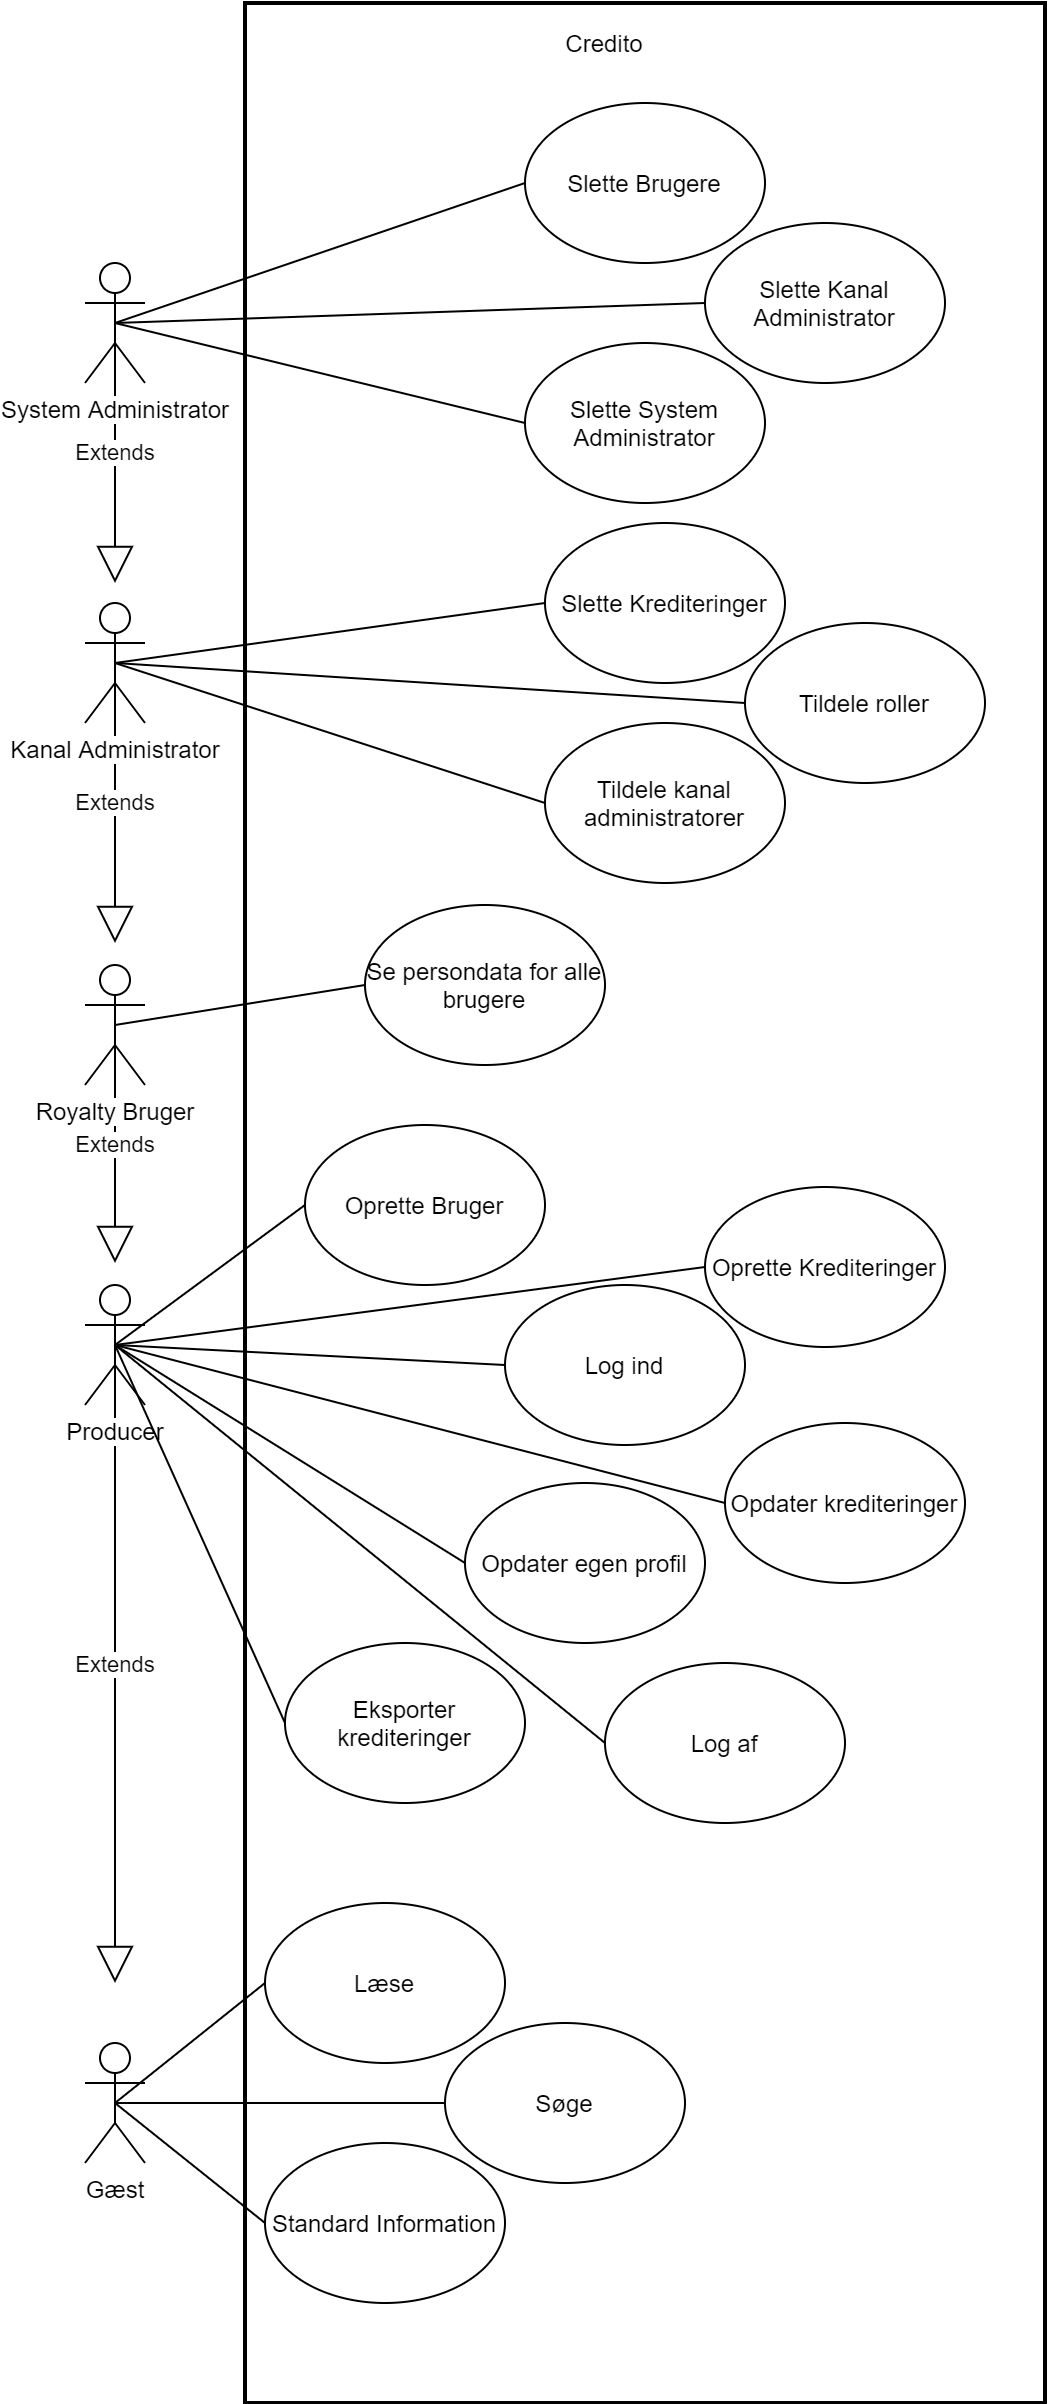
\includegraphics[scale=0.22]{figures/use-case.png}
    \caption[Overordnet brugsmønster over Creditoro systemet]%
    {Overordnet brugsmønster over Creditoro systemet 
    \par \small Menneskene er aktører. \\
    \small Cirklerne beskriver handlinger aktørne kan lave. \\
    \small Pilende betyder Extends, hvilket vil sige aktørerne arver funktionalitet}
    \label{fig:usecasemodel}
\end{figure}

% ---------------------------- Supplerende krav ------------------------------------
\subsection{Supplerende krav}

Her bruges FURPS for supplerende krav.
\begin{table}[ht]
    \begin{tabularx}{\textwidth}{|p{1cm}|X|X|}
        \hline
        \textbf{\#} &   \textbf{FURPS}           &    \textbf{Krav} \\
        \hline
        %What the customer wants! Note that this includes security-related needs.
        S01 &   Funktionalitet (Functionality)           & Skal kunne kreditere produktionsroller som er angivet af DRs Krediteringsregler \\ & & Skal overholde GDPR \\
                                
        \hline
        % How effective is the product from the standpoint of the person who must use it? Is it aesthetically acceptable? Is the documentation accurate and complete?
        S02 & Brugervenlighed (Usability)       & Systemet skal kunne understøtte flere sprog \\
        \hline
        % What is the maximum acceptable system downtime? Are failures predictable? Can we demonstrate the accuracy of results? How is the system recovered?
        S03 &   Pålidelighed (Reliability)     &  Hvis serveren til systemet genstarter, startes del-systemerne igen automatisk. Der vil ikke være behov for at ligge systemet ned regelmæssigt for at kunne foretage backup. \\
        \hline
        % How fast must it be? What's the maximum response time? What's the throughput? What's the memory consumption?
        S04 &   Ydeevne (Performance)     &  Databasen skal kunne håndtere 10000 nye brugere - samt 15000 krediteringerer årligt i 25 år, uden at ofte brugte kald til REST Api'et bliver sløvt (reponsetid på mere end 300 ms) \\
        \hline
        % Is it testable, extensible, serviceable, installable, and configurable? Can it be monitored?
        S05 & Kompabilitet (Supportability)  &  Systemet vil indeholde unit tests, og komme med en rapport over hvor stor en procendel der er dækket af dette. % Hvis der er mere tid kan vi indrage integrations tests?
        %Centraliseret logning (Elastic search, eller blot centraliseret system log?)
        Systemet vil blive forbundet til det centraliserede fejllognings system \texttt{Sentry}.
        Systemet er installerbart vha. Docker via Docker-compose. % (så vi blot kan sige docker-compose up -d for at få systemet op).
        Det vil være muligt at konfigurere system indstillinger via en \texttt{.env} (miljø) fil.
        En opsætningsguide vil være at finde sammen med kildekoden. 
        \\ \hline
    %   % Do things like I/O devices or DBMS constrain how the software must be built?
    %    Design constraints  &   Systemet skal benytte en relationel database. Databasen skal laves i PostgreSQL og skrives i programmeringssproget SQL  \\ 
    %    \hline
        % Do the programmers need to adhere to standards? Is the use of TDD required? Is statistically sound testing in the context of Cleanroom required?
    %    Implementation requirements     &    \\ 
    %   \hline 
        % What downstream feeds must be created? What other systems must this one interface with? How frequent are feeds produced?
    %   Interface requirements  &    tekst \\ 
    %   \hline 
        % What hardware must the system be deployable on? Must we be able to deploy to a machine no larger than 12" square, to be stationed in the Iraqi desert?
    %    Physical requirements   &   Ingen\\ 
    %    \hline
    \end{tabularx}
    \caption{FURPS}
    \label{tab:furps}
\end{table} 

\myworries{Følgende skal overvejes:}

\begin{itemize}
    \item Usability: Responsive UI
    \item Perfomance: The system should be able to handle 5000 concurrent users within a minute.
\end{itemize}
